The Great Work Begins!

The following content is taken from Chang and DeDeo, ``Divergence and the Complexity of Difference in Text and Culture.''

\section{Some figures and citations}

Fig. \ref{fig:operationalization_summary} summarizes our discussion up to this point. We began by distinguishing difference and distance, and pointed out the inherent limitation of distance as embodied experience. Below we shall see divergence in action. It will turn out that divergence, and the underlying epistemic notions it tracks, violates the axioms of distance---``symmetry'' and ``no shortcut'' in particular---in crucial and useful ways.

\begin{figure}[H]%[!htbp]
  \centering
  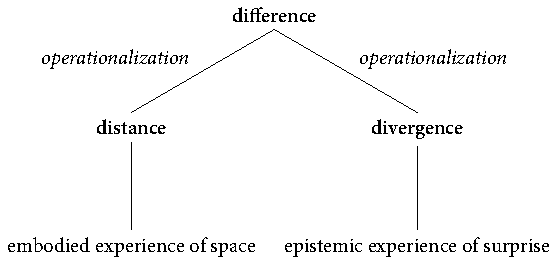
\includegraphics[width=0.75\textwidth]{fig/summary.pdf}
  \caption{Two paths to operationalizing difference: a cognitive approach made possible by the information-theoretic notion of divergence provides a different account of how things differ than the more familiar spatial metaphor of distance.}
  \label{fig:operationalization_summary}
\end{figure}

Given an interpretive frame, we can often consider one text as being broader, or ranging over more themes, than another. One can then speak of the asymmetrical relationship of one text being contained, or enclosed, by another. Consider, for example, the case of diction. At any particular time, a culture will have a range of registers available for a text to use~\autocite{bachtin2011Dialogic}. One text may have an elevated diction, another low, and a third might mix the two. A recent study by Stefania Degaetano-Ortlieb and Elke Teich shows how scientific English became broader, or gradually came to \textit{enclose}, general English over the second half of the nineteenth century.\footnote{See~\fullcite{degaetanoOrtlieb2019Optimal}, where they establish this ``subtle effect'' of scientific language enclosing general English in passing. They do so precisely in the way we argue for here, by reference the asymmetric nature of KL divergence. In their phrase, which captures the cognitive aspect of the information theoretic quantities in play, the enclosure relationship indicated by the KL asymmetry implies that general English is a worse ``model'' for scientific English than vice versa. See also~\fullcite{DegaetanoOrtlieb2019b}.} There are certainly words that are common in general English that are less common in scientific English (for example, the word ``wife''). However, there are (roughly speaking) far more words in scientific English that are rarely, if ever, used in general English (such as ``oxide''). This imbalance is measured by the Kullback--Leibler asymmetry.

\section{Some tables}

To drive this intuition, consider two major words of Russian literature, \emph{Anna Karenina} and \emph{War and Peace}, by Leo Tolstoy. In a very general sense (and the only one needed to understand this example), both of these novels deal with themes of friendship, suffering, war, and love, but in different proportions; while \emph{Anna Karenina} is most famously centered around a love story, \emph{War and Peace} follows a variety of characters as they navigate a broader array of life events.

We can represent, in this toy example, the two novels as probability distributions over these themes. Explicitly, the distributions $p_A$ (\emph{Anna Karenina}) and $p_B$ (\emph{War and Peace}) quantify the themes by reference to the relative proportions of words associated with the core concepts in order, as in table~\ref{tab:novelthemes}:\footnote{For this toy example, friendship words are: friend, friendship, companionship, fellowship, camaraderie; suffering words are: suffering, hurt, ache, pain, agony, miserable, wretched; war words are: war, conflict, warfare, combat, fighting, struggle, armed, military, bloodshed; and love words are: love, lover, fondness, tenderness, warmth, intimacy, attachment, endearment.}
\begin{eqnarray*}
p_A & =  & \{0.14, 0.21, 0.08, 0.57\}, \\
p_B & =  & \{0.15, 0.15, 0.37, 0.36 \}.
\end{eqnarray*}
Intuitively, at this level of analysis, \emph{War and Peace} covers a broader range of themes than \emph{Anna Karenina}; the latter, for example, distributes only 8\% of its coverage to war, compared to 37\% in \emph{War and Peace}.

\begin{table}[H]%[!htbp]
  \fontsize{12}{12}\selectfont
  \centering
  \begin{tabular}{@{}llll@{}}
    \toprule
    theme      & \emph{Anna Karenina} & \emph{War and Peace} \\
    \midrule
    friendship & 14\%    & 15\% \\
    suffering  & 21\%    & 12\% \\
    war        & 8\%     & 37\% \\
    love       & 57\%    & 36\% \\
    \bottomrule
  \end{tabular}
  \caption{While \emph{Anna Karenina} is dominated by words associated with love, \emph{War and Peace} has a more uniform distribution over the four themes considered here. In this sense, \emph{War and Peace} ``encloses'' the themes in \emph{Anna Karenina}, and while the Kullback--Leibler from \emph{Anna Karenina} to \emph{War and Peace} is 0.49 bits, the Kullback--Leibler in the reverse direction, from \emph{War and Peace} to \emph{Anna Karenina}, is only 0.35 bits. In this example, the compositions of the two novels are determined by counting words associated with the four themes in the English-language translations of Constance Garnett and computing the relative odds. The listed probabilities are then conditional probabilities: given that one has encountered one of these themes, what are the probabilities that it was this one or that.}\label{tab:novelthemes}
\end{table}


The Kullback--Leibler Divergence reflects these differences in the asymmetry between the two directions. The KL from \emph{Anna Karenina} to \emph{War and Peace} (i.e., ``the surprise on reading \emph{Anna Karenina} and then encountering \emph{War and Peace}, when one searches for these themes''), is $0.49$ bits, while the KL from \emph{War and Peace} to \emph{Anna Karenina} is $0.35$ bits. The enclosure relationship is captured in the asymmetry, or difference, in surprise.\footnote{Formally, our operationalization of enclosure, $\textrm{KL}(p_1|p_2)-\textrm{KL}(p_B|p_A) > 0$, indicates that $p_A$ encloses $p_B$.} In this interpretative framework, readers who begin with \emph{Anna Karenina} have little exposure to narratives involving war; when they read \emph{War and Peace}, they encounter new patterns associated with the war theme more than one third of the time. Conversely, readers who begin with \emph{War and Peace} have significant exposure to all four themes; they see less representation of some of them than they would in \emph{Anna Karenina}, but not enough to overcome the near-total absence of war in the latter. The underlying asymmetry of $0.074$ bits between the texts, in the direction from \emph{War and Peace} to \emph{Anna Karenina}, captures this relationship.
